

\newcommand{\mrspSlideBis}{%
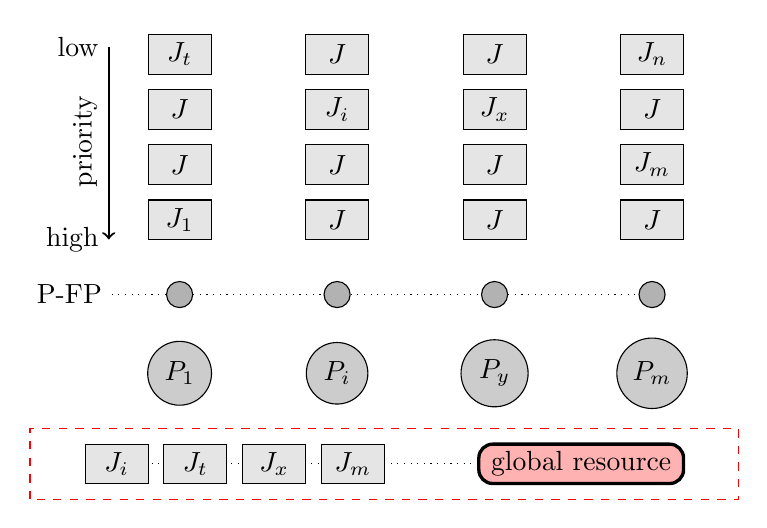
\begin{tikzpicture}[
  every text node part/.style={align=center},
  every circle node/.style={minimum width=.5ex},
  cpusty/.style={fill=gray!40,draw,circle,minimum width=1cm},
  task/.style={fill=black!10},
  sched/.style={fill=black!30,draw,circle,minimum width=1cm},
  ressty/.style={fill=red!30, draw, very thick, rounded corners=5pt}
]
%general params
\def\th{.5} %task height
\def\padding{.7}
\def\offset{.4}

% \partition{1};

  \node[cpusty] (P1) at (0+\offset,-1) {$P_1$};
  \node[sched]  (S1) at (0+\offset,0) {};

  \draw[task] (0.0,\padding*1) rectangle +(0.8, \th) node[midway,black]{$J_1$};
  \draw[task] (0.0,\padding*2) rectangle +(0.8, \th) node[midway,black]{$J$};
  \draw[task] (0.0,\padding*3) rectangle +(0.8, \th) node[midway,black]{$J$};
  \draw[task] (0.0,\padding*4) rectangle +(0.8, \th) node[midway,black]{$J_t$};

  \node[cpusty] (PI) at (2+\offset,-1) {$P_i$};
  \node[sched]  (SI) at (2+\offset,0) {};

  \draw[task] (2,\padding*1) rectangle +(0.8, \th) node[midway,black]{$J$};
  \draw[task] (2,\padding*2) rectangle +(0.8, \th) node[midway,black]{$J$};
  \draw[task] (2,\padding*3) rectangle +(0.8, \th) node[midway,black]{$J_i$};
  \draw[task] (2,\padding*4) rectangle +(0.8, \th) node[midway,black]{$J$};

  \node[cpusty] (PY) at (4.0+\offset,-1) {$P_y$};
  \node[sched]  (SY) at (4.0+\offset,0) {};

  \draw[task] (4,\padding*1) rectangle +(0.8, \th) node[midway,black]{$J$};
  \draw[task] (4,\padding*2) rectangle +(0.8, \th) node[midway,black]{$J$};
  \draw[task] (4,\padding*3) rectangle +(0.8, \th)  node[midway,black]{$J_x$};
  \draw[task] (4,\padding*4) rectangle +(0.8, \th) node[midway,black]{$J$};

  \node[cpusty] (PN) at (6.0+\offset,-1) {$P_m$};
  \node[sched]  (SN) at (6.0+\offset,0) {};

  \draw[task] (6,\padding*1) rectangle +(0.8, \th) node[midway,black]{$J$};
  \draw[task] (6,\padding*2) rectangle +(0.8, \th) node[midway,black]{$J_m$};
  \draw[task] (6,\padding*3) rectangle +(0.8, \th) node[midway,black]{$J$};
  \draw[task] (6,\padding*4) rectangle +(0.8, \th) node[midway,black]{$J_n$};
  
  \draw[dotted] (S1) -- (SI);
  \draw[dotted] (SI) -- (SY);
  \draw[dotted] (SY) -- (SN);

  \node (PFP) at (-1,0) {P-FP};
  \draw[dotted] (PFP) -- (S1);

  \draw[thick,->] (-.5,\padding*4.5) node[left,black]{low} node[rotate=90,left,xshift=-0.5cm,yshift=0.3cm]{priority} -- (-.5,\padding*1) node[left,black]{high};

  \begin{scope} [xshift=-0.8cm, yshift=-2.4cm]

  \draw[dashed, red] (-0.7,-0.2) rectangle (8.3,0.7);

  \draw[dotted] (0,0.25) -- +(5,0);
  \draw[task] (0,0) rectangle +(0.8, \th) node[midway,black]{$J_i$};
  \draw[task] (1,0) rectangle +(0.8, \th) node[midway,black]{$J_t$};
  \draw[task] (2,0) rectangle +(0.8, \th) node[midway,black]{$J_x$};
  \draw[task] (3,0) rectangle +(0.8, \th) node[midway,black]{$J_m$};

  \draw[ressty] (5,0) rectangle +(2.6,.5) node[midway]{global resource};

  % \node[inner sep=0pt] (arrow) at (8.5,1.2) {\includegraphics[width=.1\textwidth]{images/redArrow.png}};

  \end{scope}
 
\end{tikzpicture}
}

% \newcommand{\overheadsSuffered}[2]{%
% \begin{tikzpicture}[
%   xscale=#1,
%   yscale=#2,
%   every node/.append style={transform shape},
%   queuesty/.style={fill=white, very thick, font=\tiny},
%   srpsty/.style={fill=white, draw, circle, text width=.17cm, font=\tiny, very thick},
%   numsty/.style={text width=.1cm, font=\tiny},
%   arrow/.style={->},
%   littletext/.style={font=\sffamily\tiny,inner sep=0pt,outer sep=-2pt,fill=white},
%   ressty/.style={fill=red!30, draw, very thick, rounded corners=5pt},
%   emptytask/.style={rectangle, minimum width=.7cm,font=\footnotesize},
%   taskHolder/.style={fill=blue!90, draw, rectangle, minimum width=.7cm,font=\footnotesize},
%   taskWaiting/.style={fill=blue!70, draw, rectangle, minimum width=.7cm,font=\footnotesize,postaction={pattern=north east lines, very thin, pattern color=white}},
%   taskAccess/.style={fill=blue!30, draw, rectangle, minimum width=.7cm,font=\footnotesize},
%   taskNotAccess/.style={fill=white, draw, rectangle, minimum width=.7cm,font=\footnotesize}]

% \def\blockdim{(.7,.25)}

% \draw[arrow] (2.2,5.25) to[out=90,in=0] (2.35,6.6);

% \begin{scope}[xshift=2.2cm, yshift=5cm]
%   \coordinate (SRPnode) at (0,0);

%   \draw[dashed,purple] (-1.5,-0.78) -- (0.27,-0.78);

%   \node[taskNotAccess]  (T1)  at (-0.8,-0.50)  {};
%   \node[emptytask]      (TP1) at (-0.8,-0.75) {$\cdots$};
%   \node[taskWaiting]     (T2)  at (-0.8,-1.00)  {};
%   \node[emptytask]      (TP1) at (-0.8,-1.25) {$\cdots$};
%   \node[taskAccess]     (T3)  at (-0.8,-1.50)  {};
%   \node[emptytask]      (TP1) at (-0.8,-1.75) {$\cdots$};
%   \node[taskNotAccess]  (T4)  at (-0.8,-2.00)  {};
%   \node[emptytask]      (TP1) at (-0.8,-2.25) {$\cdots$};
%   \node[taskNotAccess]     (T5)  at (-0.8,-2.50)  {};

%   \draw[dashed, thin] ([shift={(-1.5,0)}]SRPnode) node[right,xshift=.1cm,littletext]{Partition$_2$} rectangle ([shift={(.3,-.15)}]T5.south-|SRPnode.east);

%   \node[srpsty] (SRP) at (SRPnode) {}; \node[font=\sffamily\tiny] at(SRPnode.west){SRP};
%   \draw[arrow] (T2.east) to[out=0,in=270] (SRP.south);

%   \draw[red] ([shift={(-.4,.17)}]T2) rectangle ([shift={(.25,-.05)}]T5.south-|T5.east);

%   \draw[arrow,red] (-0.35,-3.05) -- ([shift={(.1,-.05)}]T5.south-|T3.east);

% \end{scope}